\documentclass{article}


\usepackage{arxiv}
\usepackage{algorithm,algpseudocode}

\usepackage[utf8]{inputenc} % allow utf-8 input
\usepackage[T1]{fontenc}    % use 8-bit T1 fonts
\usepackage{hyperref}       % hyperlinks
\usepackage{url}            % simple URL typesetting
\usepackage{booktabs}       % professional-quality tables
\usepackage{amsfonts}       % blackboard math symbols
\usepackage{nicefrac}       % compact symbols for 1/2, etc.
\usepackage{microtype}      % microtypography
\usepackage{lipsum}
\usepackage{amsmath}
\usepackage{amssymb}
\usepackage{textcomp}
\usepackage[dvipsnames]{xcolor}
\usepackage{graphicx}
\usepackage{subcaption}
\usepackage{bbold}
\usepackage{bm}
\newcommand{\CO}{\mathcal{O}}
\usepackage{wrapfig}
\newcommand\subfig[2]{{Fig.~\ref{#1}{#2}}}
\newcommand\fig[1]{{Fig.~\ref{#1}}}
\usepackage[super]{nth}
\usepackage{dirtytalk}
\usepackage{braket}
%\usepackage{blindtext}
%\usepackage{tcolorbox}
%\usepackage{graphicx}

\usepackage{empheq}
\usepackage[most]{tcolorbox}
\tcbset{highlight math style={boxsep=1mm,colback=blue!30!red!10!white}}

\title{Préparation de Windows 7 pour le TP}


\author{
Pour toute question, veuillez contacter\\
 Juliane U. Klamser\\%\thanks{website}\\
  Gulliver,  ESPCI\\
  Paris \\
  \texttt{Juliane.Klamser@espci.psl.eu} \\
}

\begin{document}
\maketitle

\tableofcontents

%\begin{abstract}
%Bla bla
%\end{abstract}


% keywords can be removed
%\keywords{First keyword \and Second keyword \and More}
\section{Remarques générales}
Il existe de nombreux compilateurs C souvent gratuits (même le compilateur de MicroSoft est gratuit), nous vous proposons d'installer GCC le compilateur de GNU parce qu'il existe sur presque toutes les machines et les systèmes d'exploitation. Coder c'est bien, on peut presque tout faire, mais utiliser le travail des autres c'est encore mieux. Au-delà du compilateur, il est très commode de pouvoir bénéficier de très nombreuses librairies que d'autres, beaucoup plus courageux que vous, ont écrites. En fait, ces librairies sont en permanence améliorées et elles dépendent les unes des autres, les recopier et les garder compatibles entre elles est un challenge. 
Heureusement il existe des logiciels qui vous permettent de conserver et d'étendre une chaîne de compilation et de librairies à jour sans trop souffrir. C'est particulièrement vrai sur Linux où ils se nomment \textbf{apt-get} ou \textbf{pacman}. Sur Windows c'était beaucoup moins simple, mais il existe maintenant un logiciel qui vous permet de retrouver l’environnement style Linux pour compiler des applications Windows. C'est ce que nous vous proposons d'utiliser. Il s'agit de \textbf{MSYS2} qui va installer une console Linux sur votre Windows, cette console sera très similaire à un terminal de Linux elle vous permettra de lancer le logiciel \textbf{pacman} qui se connecte à internet et se charge d'installer et surtout de gérer automatiquement les dépendances des logiciels et librairies que vous installerez. Pour plus tard, vous trouverez peut-être ce site utile, où vous pourrez trouver toutes les bibliothèques de \textbf{pacman}: \href{https://packages.msys2.org/search}{https://packages.msys2.org/search}

Dans ce qui suit, nous allons décrire comment installer un compilateur associé à un jeu de librairies de fonctions. Cet outil vous permettra de « compiler » un programme que vous aurez écrit et qui utilisera éventuellement des librairies faites par d'autres. Ce compilateur est un programme qui fonctionne à la ligne de commande, c'est assez rudimentaire, mais cela permet de faire beaucoup de choses. Vous aurez également besoin d'un éditeur qui permet d'écrire votre programme (comme Word ou LibreOffice vous permettent d'écrire une lettre). Si vous utilisez déjà un éditeur et qu'il est adapté au langage C continuez à l'utiliser. Si non, vous trouverez plus tard (chapitre \ref{S:Editor}) quelques propositions pour un éditeur de code.

Dans le texte qui suit vous trouverez une description étape par étape de l'installation, en principe si vous suivez cette recette cela devrait marcher. En pratique, vous pouvez disposer d'un ordinateur avec une configuration particulière et il est possible qu'une étape demande un ajustement. Avant de décrire la recette, voici la philosophie de notre installation. 

D'abord MSYS2 peut paraitre un peu plus compliqué à installer, car ce système est évolutif, vous trouverez d'autres versions de GCC qui s'installent en une opération, mais il est très difficile de rajouter des librairies et encore plus de les mettre à jour. L'installation de MSYS2 se fait en plusieurs étapes :
\begin{enumerate}
\item une console du style Unix
\item sa mise à jour
\item l'installation du compilateur 64 bits
\item la possibilité d'aller plus loin.
\end{enumerate}
 
 \section{Type de système : 32 bits ou 64 bits ?}
 Avant de commencer, il faut déterminer quelle est la version de Windows sur votre PC : est-ce un OS 32 ou un 64 bits ? En principe, de nos jours vous devriez avoir un OS 64 bits, mais ce n'est pas inutile de vérifier. Pour ce faire aller dans le menu « démarrer », placer votre souris au-dessus de « ordinateur » et faites un click \textbf{droit} et cliquer sur propriétés, vous devez voir apparaître une fenêtre disant :
 \begin{figure}[H]
\begin{subfigure}[c]{0.5\textwidth}
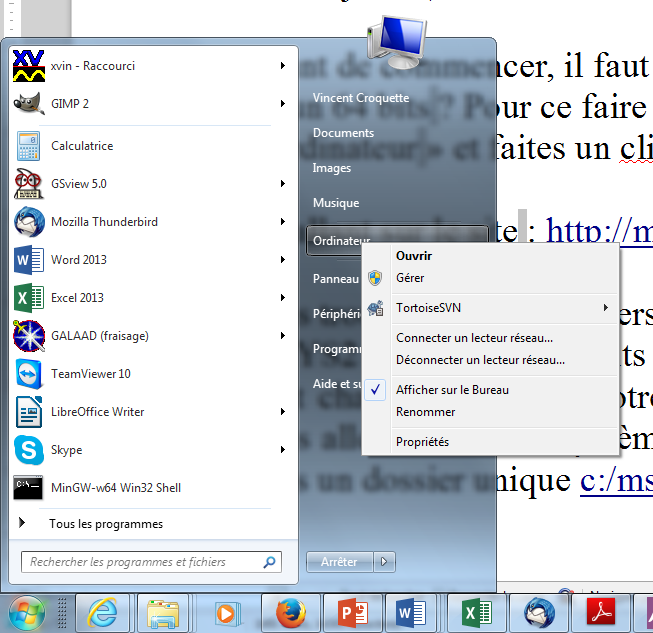
\includegraphics[width=0.95\textwidth]{Plots/Pic1.png}
\subcaption{« démarrer » $\rightarrow$ click \textbf{droit} sur « ordinateur » $\rightarrow$ propriétés}
\end{subfigure}
\begin{subfigure}[c]{0.5\textwidth}
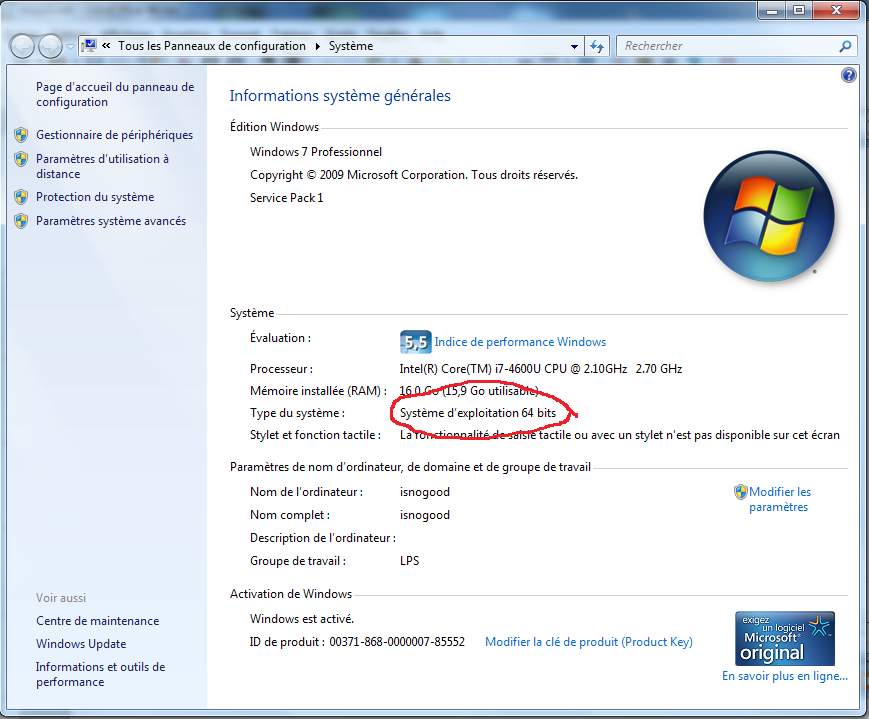
\includegraphics[width=0.95\textwidth]{Plots/Pic2.png}
\subcaption{l'information requise est marquée en rouge}
\end{subfigure}
\caption{Trouver votre type de système.}
\end{figure}

\section{Installation de MSYS2}
\subsection{Installation de la console Unix}
Durant toute l'installation, vous devez être connecté à internet. En allant sur le site : \href{http://msys2.github.io/}{http://msys2.github.io/} vous trouverez des liens vers : MSYS2 en version 32 bits ou MSYS2 en version 64 bits (voir l'image ci-dessous). Suivant votre système, chargez l'un ou l'autre et exécutez cet installeur. Ce faisant vous allez installer le système minimal permettant de démarrer, tous les fichiers utiles seront situés dans un dossier unique c:\textbackslash msys32 ou c:\textbackslash msys64
\begin{figure}[H]
\center
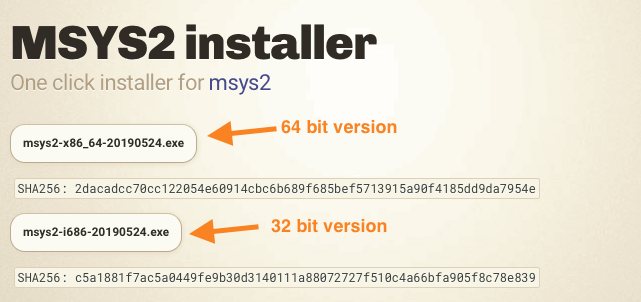
\includegraphics[width=1\textwidth]{Plots/Msys2_0.png}
\caption{Choisissez la version qui est compatible avec votre ordinateur.}
\end{figure}
Lancez le processus d'installation.\\
La description de l'installation est bien faite sur la page de MSYS2. Néanmoins, vous trouverez peut-être utile ce qui suit.

Votre processus d'installation devrait être comparable à la \fig{F:installationMsys2}.
 \begin{figure}[H]
\begin{subfigure}[c]{0.5\textwidth}
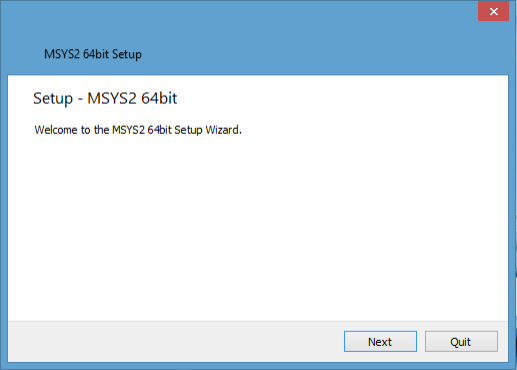
\includegraphics[width=0.95\textwidth]{Plots/Msys2_1.png}
\subcaption{ étape 1\newline\newline\newline\newline\newline\newline\newline}
\end{subfigure}
\begin{subfigure}[c]{0.5\textwidth}
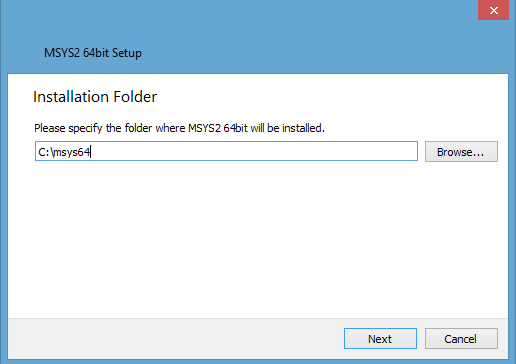
\includegraphics[width=0.95\textwidth]{Plots/Msys2_2.png}
\subcaption{ étape 2: Le plus simple est de choisir les options d'installation par défaut. Cependant, si vous savez ce que vous faites, vous pouvez choisir le dossier où vous souhaitez installer votre logiciel, par exemple c:\textbackslash msys64 si vous avez un système 64 bits c:\textbackslash msys32 sinon. Vous pouvez choisir un autre nom ou installer MSYS2 sur un autre disque (ex. d:\textbackslash msys64), mais surtout ne choisissez pas un nom compliqué ou contenant un espace ! Choisissez un endroit où vous avez le droit d'écrire (surtout pas c:\textbackslash Program Files).}
\end{subfigure}
\begin{subfigure}[c]{0.5\textwidth}
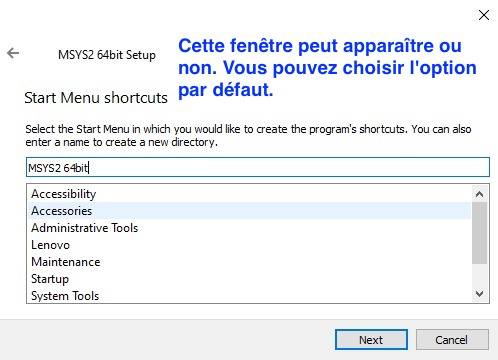
\includegraphics[width=0.95\textwidth]{Plots/Msys2_3.jpeg}
\subcaption{ étape 3 : Cette fenêtre peut apparaître ou non. Vous pouvez choisir l'option par défaut.}
\end{subfigure}
\begin{subfigure}[c]{0.5\textwidth}
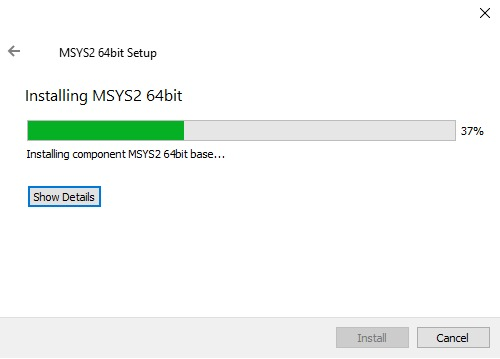
\includegraphics[width=0.95\textwidth]{Plots/Msys2_4.jpeg}
\subcaption{ étape 4 : Attendez que l'installation soit terminée.\newline}
\end{subfigure}
\begin{subfigure}[c]{0.5\textwidth}
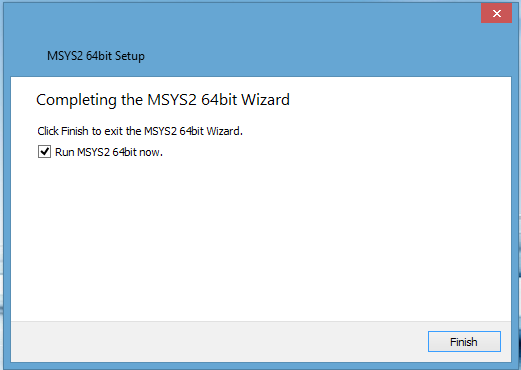
\includegraphics[width=0.95\textwidth]{Plots/Msys2_5.png}
\subcaption{ étape 5}
\end{subfigure}
\begin{subfigure}[c]{0.5\textwidth}
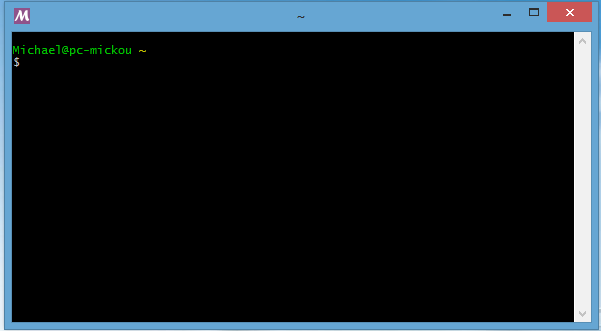
\includegraphics[width=0.95\textwidth]{Plots/Msys2_6Terminal.png}
\subcaption{ étape 6: En cliquant sur Finish, vous devriez voir apparaître la console MSYS2 Shell.}
\end{subfigure}
\caption{Comment l'installation ressemblerait le plus probablement pour vous.\label{F:installationMsys2}}
\end{figure}


\subsection{Mise à jour de MSYS2}
He oui, à peine installer il faut mettre à jour, pour cela recopier la ligne de commande ci-dessous (dans le champ noir) et coller la dans la console (click droit, paste). Confirmez avec ENTER !
\begin{tcolorbox}[width=\textwidth,colframe=Purple,colback={black},title={Ceci est la console MSYS2 Shell},outer arc=0mm,colupper=white]    
      pacman --needed -Sy bash pacman-mirrors msys2-runtime
\end{tcolorbox}
Vous devriez voir apparaître quelque chose comme dans la \fig{F:firstPaxman}.
\begin{figure}[H]
\center
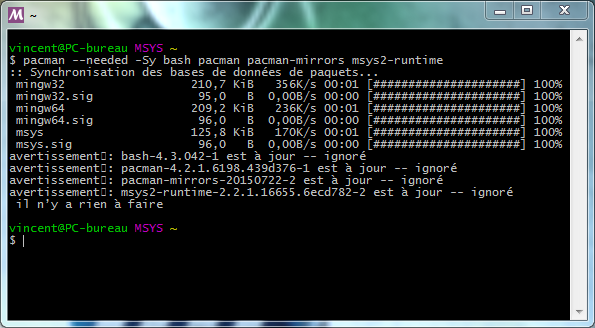
\includegraphics[width=0.75\textwidth]{Plots/Msys2_7Terminal.png}
\caption{Résultat de pacman --needed -Sy bash pacman-mirrors msys2-runtime.\label{F:firstPaxman}}
\end{figure}
À ce stade, vous devez mettre à jour le logiciel et sa base de données en tapant (il faut être connecté à internet pour que cela marche):
\begin{tcolorbox}[width=\textwidth,colframe=Purple,colback={black},title={Ceci est la console MSYS2 Shell},outer arc=0mm,colupper=white]    
      pacman -Syu
\end{tcolorbox}
Vous devriez voir apparaître quelque chose comme dans la \fig{F:2Paxman}.
\begin{figure}[H]
\center
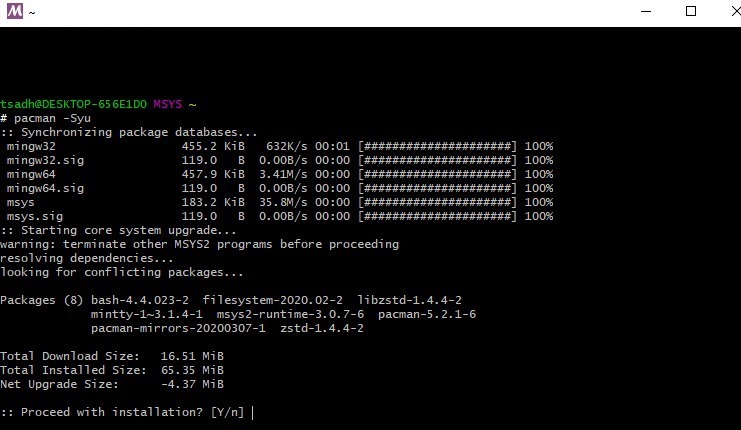
\includegraphics[width=0.75\textwidth]{Plots/Msys2_8Terminal.jpeg}
\caption{Résultat de pacman -Syu.\label{F:2Paxman}}
\end{figure}
Tapez la majuscule Y et appuyez sur ENTER pour continuer. Attendez que l'installation soit terminée. 

Note: \textbf{Il est possible que le premier essai ne se termine pas avec succès.} Dans ce cas, la console vous indiquera des lignes avec "warning : ...". Lisez le warning et essayez de suivre les instructions. Il vous demandera probablement simplement de fermer la console MSYS2 Shell et de répéter la commande pacman -Syu.

\textbf{Un résultat réussi} devrait ressembler à la \fig{F:Syu} (il n'y a pas de warnings !).
\begin{figure}[H]
\center
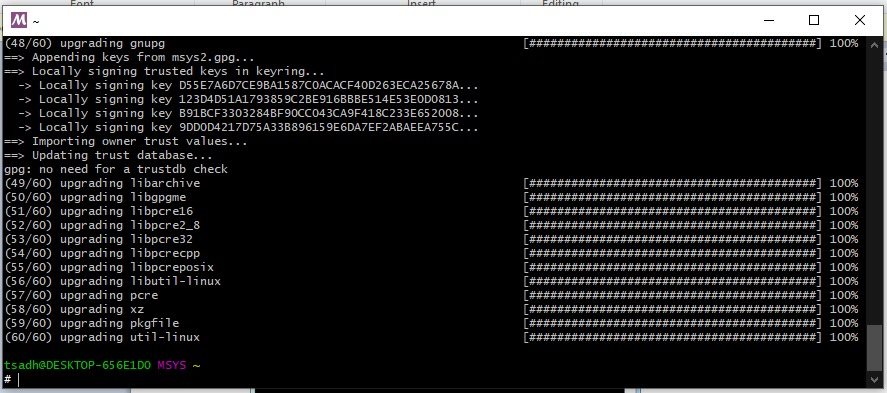
\includegraphics[width=0.75\textwidth]{Plots/Msys2_9Terminal.jpeg}
\caption{Un résultat réussi de pacman -Syu.\label{F:Syu}}
\end{figure}
Pour tester si votre installation est réussie. Tapez
\begin{tcolorbox}[width=\textwidth,colframe=Purple,colback={black},title={Ceci est la console MSYS2 Shell},outer arc=0mm,colupper=white]    
      pacman -Su
\end{tcolorbox}
Vous devriez obtenir un résultat comme indiqué dans la \fig{F:Su}.
\begin{figure}[H]
\center
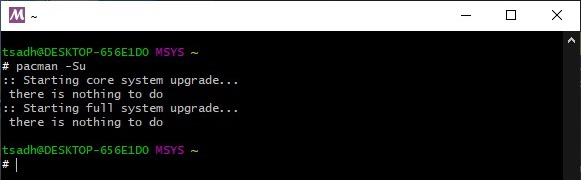
\includegraphics[width=0.75\textwidth]{Plots/Msys2_9b.jpeg}
\caption{Un résultat réussi de pacman -Su.\label{F:Su}}
\end{figure}
Vous avez mis à jour la base des paquets de logiciels de votre installation.

À ce stade vous avez installé le logiciel MSYS2 qui contient \textbf{3 consoles} et tout ce qu'il faut pour installer et mettre à jour d'autres «paquets» c'est-à-dire des ensembles de logiciels et de librairies. Si vous cliquez sur «démarrer $\rightarrow$ tous mes programmes» vous allez voir apparaître ceci (\fig{F:FindMsys2}):
\begin{figure}[H]
\center
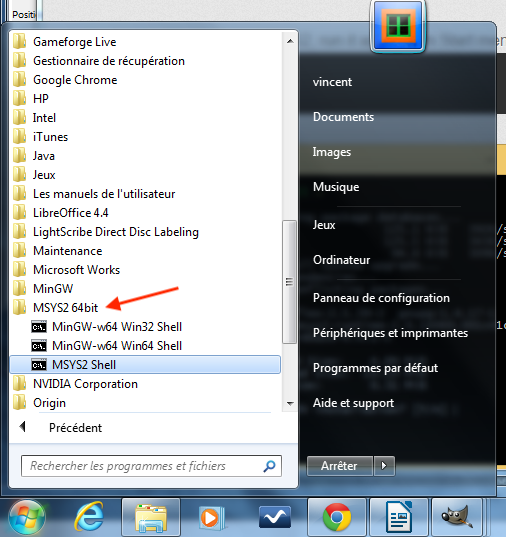
\includegraphics[width=0.5\textwidth]{Plots/Msys2_10Start.png}
\caption{Où trouver les consoles.\label{F:FindMsys2}}
\end{figure}

Ce sont les trois consoles (Shell en anglais) dont nous venons de parler, en cliquant sur leur nom elles se lancent.  

La console {\color{Purple}\textbf{MSYS2 Shell}} permet de procéder aux installations et aux mises à jour de tous les paquets de logiciels. Ceux-ci sont de deux types 32 bits et 64 bits.

La console \textbf{MinGW-w64 Win32 Shell} permet de travailler avec tous les paquets en 32bits.

La console {\color{MidnightBlue}\textbf{MinGW-w64 Win64 Shell}} permet de travailler avec tous les paquets en 64bits.

\subsection{Installation du compilateur en 64 bits}
Vous pouvez maintenant installer le compilateur. L'outil MSYS2 permet de travailler en 64 bits.\\\underline{Sur une machine 32 bits} vous pourrez compiler et exécuter du 32bits, vous pourrez compiler des applications 64 bits, mais elles ne tourneront pas sur votre machine 32 bits. \\\underline{Avec une machine 64 bits}, vous pourrez compiler et exécuter des applications 32 bits et 64 bits. 

Nous proposons de travailler avec des applications 64 bits. MSYS2 vous propose deux terminaux différents: \textbf{MinGW-w64 Win32 Shell} et \textbf{MinGW-w64 Win64 Shell}, qui vous permettent de compiler des applications 32 bits et 64 bits. {\color{MidnightBlue}\textbf{Nous utiliserons MinGW-w64 Win64 Shell.}}

Mais si vous avez une machine 32 bits, utilisez le compilateur et la Shell en 32 bits.

\begin{tcolorbox}[width=\textwidth,colframe=black,colback={white},title={Quelques rudiments de l'utilisation de la ligne de commande dans une console.},outer arc=0mm,colupper=black]    
      Dans la console vous tapez des commandes suivies d'options éventuelles et vous exécuter cette commande en pressant ENTER: \\
\newline
\textbf{ls} par exemple va lister les fichiers dans le dossier courant en donnant uniquement leurs noms. \\
\textbf{ls -l} va lister les fichiers avec plus d'informations.\\
\newline
\textbf{pacman} et la commande qui est au cœur du système MSYS2, elle vous permet de rechercher des logiciels puis de les installer en installant également toutes les dépendances. Par la suite elle vous permettra de les mettre à jour. Ici, vous pouvez rechercher des logiciels/paquets \href{https://packages.msys2.org/search}{https://packages.msys2.org/search}.
\end{tcolorbox}
 
MSYS2 possède un défaut, les noms des paquets sont assez cryptiques, ceci provient du fait qu'ils existent en plusieurs versions (32 et 64 bits), mais aussi que les paquets sont souvent regroupés pour une action particulière.

Pour installer le compilateur GCC en 64 bits, copiez la commande suivante dans la console MSYS2 Shell utilisé précédemment et confirmez avec ENTER 
\begin{tcolorbox}[width=\textwidth,colframe=Purple,colback={black},title={Ceci est la console MSYS2 Shell},outer arc=0mm,colupper=white]    
      pacman -S mingw-w64-x86\_64-toolchain
\end{tcolorbox}
Le résultat devrait ressembler à ceci (\fig{F:GNUInstall1}). Confirmez avec ENTER pour télécharger tous les paquets par défaut. Attendez ensuite que le téléchargement se termine.
\begin{figure}[H]
\center
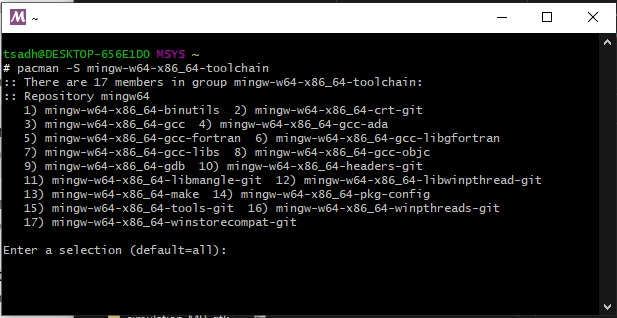
\includegraphics[width=0.75\textwidth]{Plots/Msys2_11GNU.jpeg}
\caption{Un résultat réussi de pacman -S mingw-w64-x86\_64-toolchain.\label{F:GNUInstall1}}
\end{figure}
Lorsque le téléchargement est terminé, vous devriez voir quelque chose comme dans l'image ci-dessous (\fig{F:GNUInstall2}). Appuyez sur la touche Y majuscule pour procéder à l'installation et attendez que l'installation soit terminée.
\begin{figure}[H]
\center
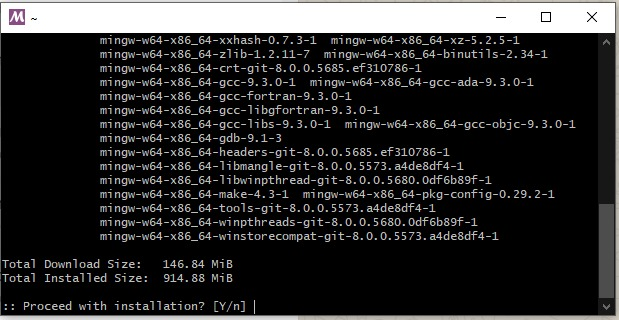
\includegraphics[width=0.75\textwidth]{Plots/Msys2_12Gnu.jpg}
\caption{Appuyez sur la touche Y majuscule pour procéder à l'installation.\label{F:GNUInstall2}}
\end{figure}
Le processus va prendre un peu de temps, l'ordre en question installe tous les paquets utiles à la compilation des programmes ce qui correspond au chargement de 105Mo soit 609,9 Mo installé au final sur votre PC. Si le processus se passe mal, vous pouvez arrêter la console, la relancer et relancer l'ordre d'installation.

À la fin vous avez installé le compilateur. Pour vérifier que l'installation est bonne, lancer la console {\color{MidnightBlue}\textbf{MinGW-w64 Win64 Shell}}, une nouvelle fenêtre devrait apparaître tapez la commande 
\begin{tcolorbox}[width=\textwidth,colframe=MidnightBlue,colback={black},title={Ceci est la console MinGW-w64 Win64 Shell},outer arc=0mm,colupper=white]    
      gcc -v
\end{tcolorbox}
(ce qui veut dire lance le compilateur gcc qui m'indique son numéro de version). Vous devriez obtenir un résultat comme dans la \fig{F:gccVersion}. Cela veut dire que vous avez la version 9.3.0 de gcc et que tout va bien. Si vous avez  quelque chose comme \textbf{gcc command not found}, c'est que l'installation n'a pas marché et il faut la reprendre.
\begin{figure}[H]
\center
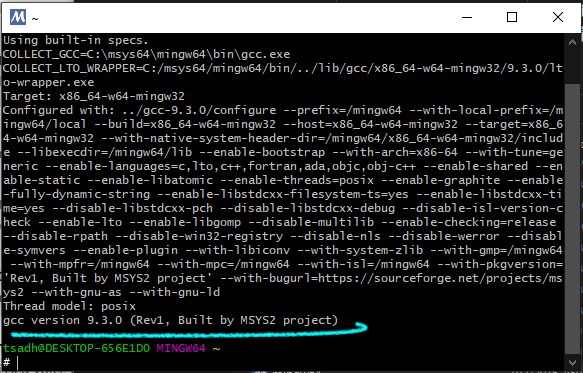
\includegraphics[width=0.75\textwidth]{Plots/Msys2Con_13Gnu.jpg}
\caption{Resultat de gcc -v.\label{F:gccVersion}}
\end{figure}


Quand vous avez un compilateur qui marche vous pouvez installer les autres librairies en tapant dans la console {\color{Purple}\textbf{MSYS2 Shell}} (attention, changement de console):
\begin{tcolorbox}[width=\textwidth,colframe=Purple,colback={black},title={Ceci est la console MSYS2 Shell},outer arc=0mm,colupper=white]    
      pacman -S mingw-w64-x86\_64-pkg-config mingw-w64-x86\_64-gtk3 make
\end{tcolorbox}
Le résultat devrait ressembler à la figure \ref{F:gtkInstal}. Là encore, vous devez confirmer le processus d'installation avec la majuscule Y. Attendez que l'installation soit terminée.
\begin{figure}[H]
\center
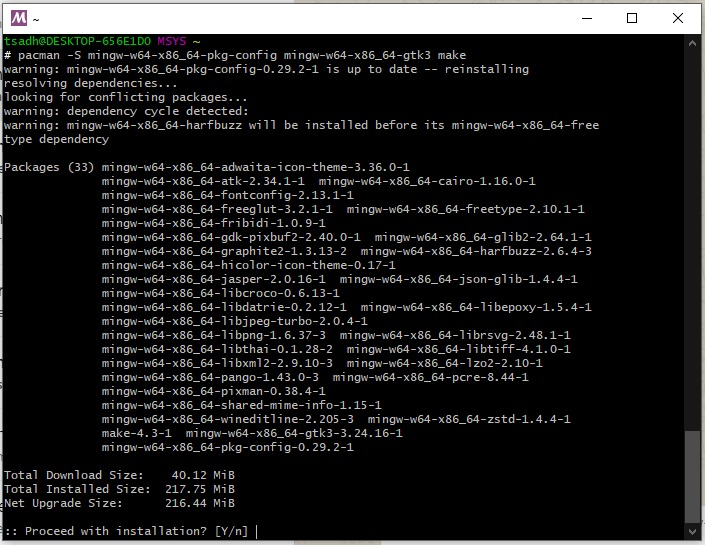
\includegraphics[width=0.75\textwidth]{Plots/Msys2_14pkg.jpg}
\caption{Resultat de pacman -S mingw-w64-x86\_64-pkg-config mingw-w64-x86\_64-gtk3 make\label{F:gtkInstal}}
\end{figure}

\section{Éditeur de code\label{S:Editor}}
Vous avez plusieurs choix.
\subsection{Notepad++}
Une façon simple de commencer et d’utiliser un éditeur de texte pour modifier le code source de vos programmes puis de compiler ce code dans la Shell. Vous pouvez installer Nodepad++ qui est léger est assez efficace, d'ici \href{https://notepad-plus-plus.org}{https://notepad-plus-plus.org}. Assurez-vous que vous installez une version compatible avec votre ordinateur.
\begin{figure}[H]
\center
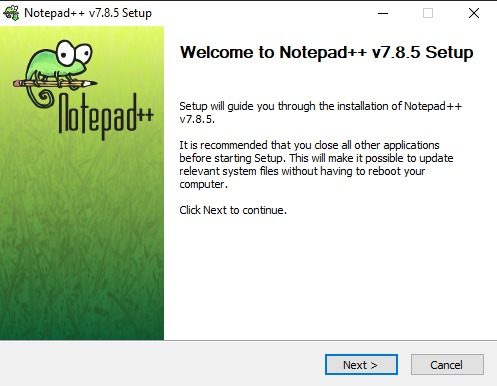
\includegraphics[width=0.4\textwidth]{Plots/Editor_1.jpg}
%\caption{Resultat de pacman -S mingw-w64-x86\_64-pkg-config mingw-w64-x86\_64-gtk3 make}
\end{figure}
\subsection{Atom}
Vous pouvez essayer atom \href{https://atom.io}{https://atom.io}\\

Ce éditeur offre une option qui vous permettent de travailler simultanément sur le même code avec quelqu'un. C'est très utile pour le projet final, lorsque vous travaillez avec un partenaire sur le même code. Cette fonction est appelée "Teletype".
\subsection{VIM ou emacs}
Il existe des éditeurs plus compliqués comme VIM. Ces éditeurs sont très puissants, ils permettent de compiler le programme dans une de leur fenêtre et il est alors possible de cliquer sur la ligne que le compilateur indique comme erronée pour y arriver directement. Ceci s’avère très pratique. Cependant, elle a besoin d'un peu de formation.

Suivez ce lien pour accéder à un tutoriel vim \href{https://www.openvim.com}{https://www.openvim.com}.

Vous obtenez VIM en tapant: 
\begin{tcolorbox}[width=\textwidth,colframe=Purple,colback={black},title={Ceci est la console MSYS2 Shell},outer arc=0mm,colupper=white]    
      pacman –S vim
\end{tcolorbox}
Pour emacs tapez 
\begin{tcolorbox}[width=\textwidth,colframe=Purple,colback={black},title={Ceci est la console MSYS2 Shell},outer arc=0mm,colupper=white]    
      pacman –S mingw-w64-x86\_64-emacs
\end{tcolorbox}

\subsection{Code::Blocks}
Si vous préférer un environnement intégré de compilation vous pouvez installer l'IDE Code::Blocks qui vous permet d'éviter la ligne de commande si vous êtes allergique et d'écrire et de compiler vos programmes dans un environnement intégrer (IDE).

Vous trouverez une description de cet IDE à cette adresse \href{http://www.codeblocks.org/}{http://www.codeblocks.org/}

Vous pouvez télécharger le logiciel à cette adresse \href{http://www.codeblocks.org/downloads}{http://www.codeblocks.org/downloads}

\section{Lançons votre premier code C.}
Rendez-vous sur ce site \href{https://github.com/JulianeUta/MD2020/blob/master/MyFirstCode.zip}{https://github.com/JulianeUta/MD2020/blob/master/MyFirstCode.zip} et cliquez sur Download. Un dossier compressé avec votre premier code en C sera téléchargé. L'objectif est de compiler le code et de l'exécuter.
\begin{figure}[H]
\center
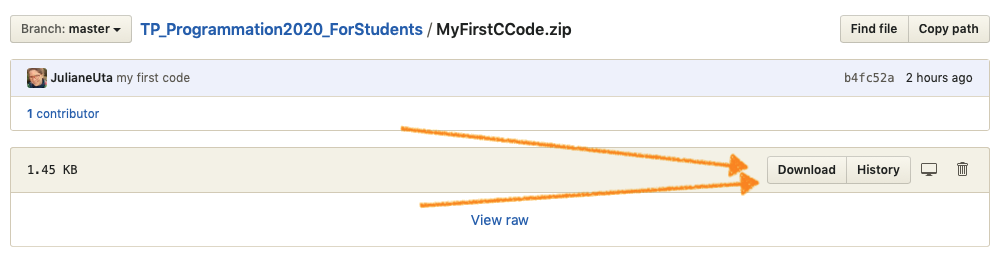
\includegraphics[width=0.6\textwidth]{Plots/FirstCode_1.png}
%\caption{Resultat de pacman -S mingw-w64-x86\_64-pkg-config mingw-w64-x86\_64-gtk3 make}
\end{figure}
Supposons que vous ayez choisi de sauvegarder le dossier compressé dans votre dossier Documents. Ensuite, allez dans votre dossier Documents et faites un clic droit sur le dossier compressé MyFirstCCode, puis sélectionnez quelque chose comme "Extraire tout...".
\begin{figure}[H]
\center
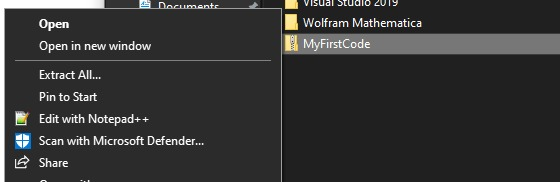
\includegraphics[width=0.6\textwidth]{Plots/FirstCode_2.jpg}
%\caption{Resultat de pacman -S mingw-w64-x86\_64-pkg-config mingw-w64-x86\_64-gtk3 make}
\end{figure}
Il devrait y avoir un dossier normal appelé MyFistCode. Allez dans ce dossier. Il y a peut-être un dossier appelé \_MACOSX.  Vous pouvez supprimer ce dossier \_MACOSX (car ce n'est qu'un artefact de la compression des dossiers sur un ordinateur avec un système d'exploitation différent). Ouvrez le fichier main.c avec Notepad++. C'est votre code. Il devrait ressembler à ceci. 
\begin{figure}[H]
\center
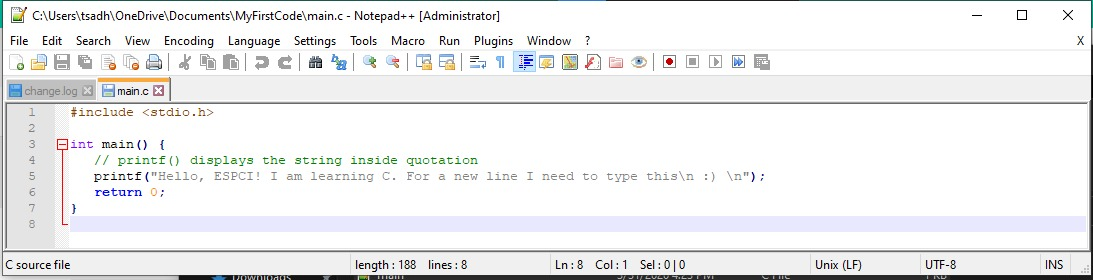
\includegraphics[width=0.95\textwidth]{Plots/FirstCode_9.jpeg}
%\caption{Resultat de pacman -S mingw-w64-x86\_64-pkg-config mingw-w64-x86\_64-gtk3 make}
\end{figure}
Nous voulons maintenant compiler le code (traduire ces mots écrits en quelque chose qui puisse être interprété par l'ordinateur). {\color{Bittersweet}\textbf{Soyez attentifs, car c'est ce que vous ferez de manière extensive pendant ce TP.}}

Faites un clic droit sur le dossier MyFirstCode et sélectionnez les propriétés. Nous devons connaître la localisation du dossier avec votre code. Dans l'exemple de la \fig{F:FindFolderAddress}, l'adresse dont nous avons besoin se trouve dans le carré bleu (voir \subfig{F:FindFolderAddress}{b}).
\begin{figure}[H]
\begin{subfigure}[c]{0.5\textwidth}
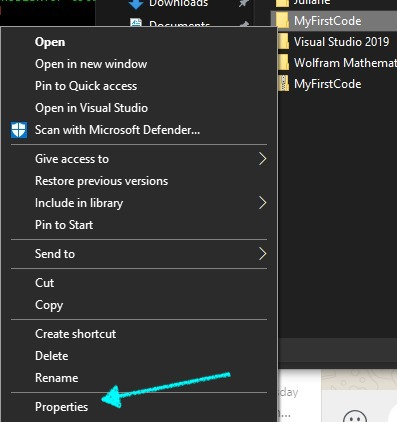
\includegraphics[width=0.75\textwidth]{Plots/FirstCode_3Properties.jpg}
\subcaption{clic droit sur MyFirstCode et sélectionnez les propriétés}
\end{subfigure}
\begin{subfigure}[c]{0.5\textwidth}
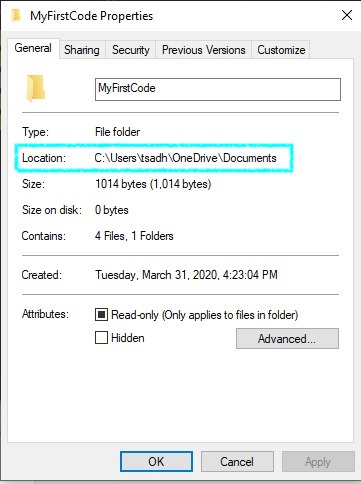
\includegraphics[width=0.75\textwidth]{Plots/FirstCode_4Path.jpg}
\subcaption{Adresse du dossier MyFirstCode}
\end{subfigure}
\caption{Comment trouver l'adresse du dossier.\label{F:FindFolderAddress}}
\end{figure}
Nous utilisons les informations contenues dans le carré bleu et les convertissons en une adresse « bash », où les noms de dossiers sont séparés par / et non par \textbackslash. Dans l'exemple donné, l'adresse « bash » correspondante est (veuillez comparer avec le carré bleu et adapter votre adresse en conséquence) \textbf{/c/Users/tsadhu/OneDrive/Documents/MyFirstCode}

Nous utilisons maintenant la console {\color{MidnightBlue}\textbf{MinGW-w64 Win64 Shell}} et naviguons vers ce dossier en tapant
\begin{tcolorbox}[width=\textwidth,colframe=MidnightBlue,colback={black},title={Ceci est la console MinGW-w64 Win64 Shell},outer arc=0mm,colupper=white]    
      cd /c/Users/tsadhu/OneDrive/Documents/MyFirstCode
\end{tcolorbox}
Si vous tapez maintenant 
\begin{tcolorbox}[width=\textwidth,colframe=MidnightBlue,colback={black},title={Ceci est la console MinGW-w64 Win64 Shell},outer arc=0mm,colupper=white]    
      ls
\end{tcolorbox}
ce qui signifie qu'il faut lister tous les fichiers de ce dossier (c'est bien un minuscule L et non un I majuscule). Vous devriez voir une sortie comme celle-ci.
\begin{figure}[H]
\center
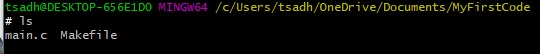
\includegraphics[width=0.9\textwidth]{Plots/FirstCode_5.jpeg}
\end{figure}
Pour compiler le code, que vous avez vu dans votre éditeur du code, tapez
\begin{tcolorbox}[width=\textwidth,colframe=MidnightBlue,colback={black},title={Ceci est la console MinGW-w64 Win64 Shell},outer arc=0mm,colupper=white]    
      make
\end{tcolorbox}
Vous devriez voir une sortie comme celle-ci.
\begin{figure}[H]
\center
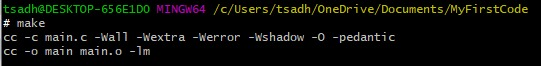
\includegraphics[width=0.9\textwidth]{Plots/FirstCode_6.jpeg}
\end{figure}
Si vous tapez maintenant 
\begin{tcolorbox}[width=\textwidth,colframe=MidnightBlue,colback={black},title={Ceci est la console MinGW-w64 Win64 Shell},outer arc=0mm,colupper=white]    
      ls
\end{tcolorbox}
Vous devriez voir une sortie comme celle-ci. Il existe deux autres fichiers, main.o et main.exe. main.exe est écrit dans une langue que l'ordinateur peut interpréter et exécuter. C'est ce que l'on appelle l'exécutable.
 \begin{figure}[H]
\center
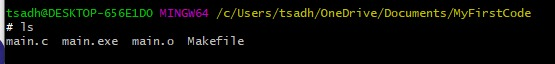
\includegraphics[width=0.9\textwidth]{Plots/FirstCode_7.jpeg}
\end{figure}
Pour exécuter le main.exe, tapez
\begin{tcolorbox}[width=\textwidth,colframe=MidnightBlue,colback={black},title={Ceci est la console MinGW-w64 Win64 Shell},outer arc=0mm,colupper=white]    
      ./main.exe
\end{tcolorbox}
Vous devriez voir une sortie comme celle-ci. 
\begin{figure}[H]
\center
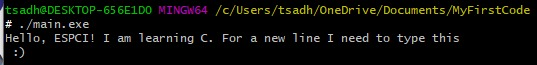
\includegraphics[width=0.9\textwidth]{Plots/FirstCode_8.jpeg}
\end{figure}
Il s'agit de la sortie du code. Si vous voyez ce résultat, alors félicitations à vous. Vous êtes maintenant prêt à commencer le TP.
\section{Gnuplot}
Gnuplot est un logiciel qui sert à produire des représentations graphiques en deux ou trois dimensions de fonctions numériques ou de données. Il sera très utile pour tracer des données avec quelques lignes. Vous pouvez télécharger Gnuplot à partir de ce site. \href{http://www.gnuplot.info/download.html}{http://www.gnuplot.info/download.html} 

Téléchargez et exécutez l'installateur. Si possible, choisissez les paramètres par défaut. Si vous le souhaitez, vous pouvez choisir le même répertoire que pour l'installation de MSYS2. Une fois l'installation terminée, vous pouvez trouver l'application gnuplot parmi vos programmes. 



%\bibliographystyle{unsrt}  
%\bibliography{references}  %%% Remove comment to use the external .bib file (using bibtex).
%%% and comment out the ``thebibliography'' section.

\end{document}
